\documentclass[aps,onecolumn,twoside,secnumarabic,balancelastpage,amsmath,amssymb,nofootinbib,hyperref=pdftex]{revtex4}


\usepackage{color}         % produces boxes or entire pages with colored backgrounds
\usepackage{graphics}      % standard graphics specifications
\usepackage[pdftex]{graphicx}      % alternative graphics specifications
\usepackage{longtable}     % helps with long table options
\usepackage{amsmath}
\usepackage{epsf}          % old package handles encapsulated post script issues
\usepackage{bm}            % special 'bold-math' package
\usepackage{verbatim}			% for comment environment                                   
\usepackage[demo]{graphicx}
\usepackage{caption}
\usepackage{subcaption}             

\usepackage[colorlinks=true]{hyperref}  % this package should be added after all others % use as follows: \url{http://web.mit.edu/8.13}                      

\begin{document}
\title{Proton Decay Opportunities at DUNE}
\author         {Noah Steinberg}
\email          {nastein@umich.edu}
\date{\today}
\affiliation{University of Michigan - Physics}

\maketitle

\section{Current limits on Proton Decay}
The best current limits on proton decay are set by Super-Kamiokande (Super-K). Super-K is a 50 kiloton (22.5 kiloton fiducial) water cherenkov detector within the Kamioka mine in Japan which has a combined exposure of more than 300 kiloton-years$^{[1]}$. In Super-K, proton decay can come from a free proton in hydrogen, or from a bound proton in oxygen. In bound protons, Fermi momentum, multi-nucleon correlations, nuclear binding energy, and decay product interactions with other nucleons smear the final state kinematics. These must be taken into account in the search for proton decay. Two decay channels, $p \rightarrow e^{+}\pi^{0}$ and $p \rightarrow K^{+}\bar{\nu}$ are discussed, with focus on the second. 

\subsection{$p \rightarrow e^{+}\pi^{0}$}

In typical GUT's the dominant channel for proton decay is $p \rightarrow e^{+}\pi^{0}$. This channel is well suited for detection by Super-K$^{[2]}$ as all final state particles are above cherenkov threshold and the distinct signal is 3 cherenkov rings, one belonging to the positron, and two belonging to the two photons from the $\pi^{0}$ decay. Backgrounds arise from interactions by atmospheric neutrino interactions which produce mesons in the detector. Cuts to isolate proton decay require$^{[2]}$:

\begin{enumerate}
\item 2 to 3 electron like cherenkov rings
\item no Michel electrons
\item $\pi^{0}$ invariant mass should be between $85 < M_{\pi^{0}} < 185$ MeV/$c^{2}$
\item total invariant mass should be between $800 < M_{tot} < 1050$ MeV/$c^2$ with total momentum less then 250 MeV/c
\item no 2.2 MeV $\gamma$ from neutron capture (neutrons are often produced in atmospheric neutrino interactions).
\end{enumerate}

For this decay channel the average signal efficiency is $\approx 38.7$ percent with an expected background of 0.61 events. As of 2017, no proton decay has been observed in this channel and a lower lifetime limit is given as $\tau/B_{p\rightarrow e^{+}\pi^{0}} > 1.6 \times 10^{34}$ yr$^{[2]}$.

\begin{figure}[htbp]
\begin{center}
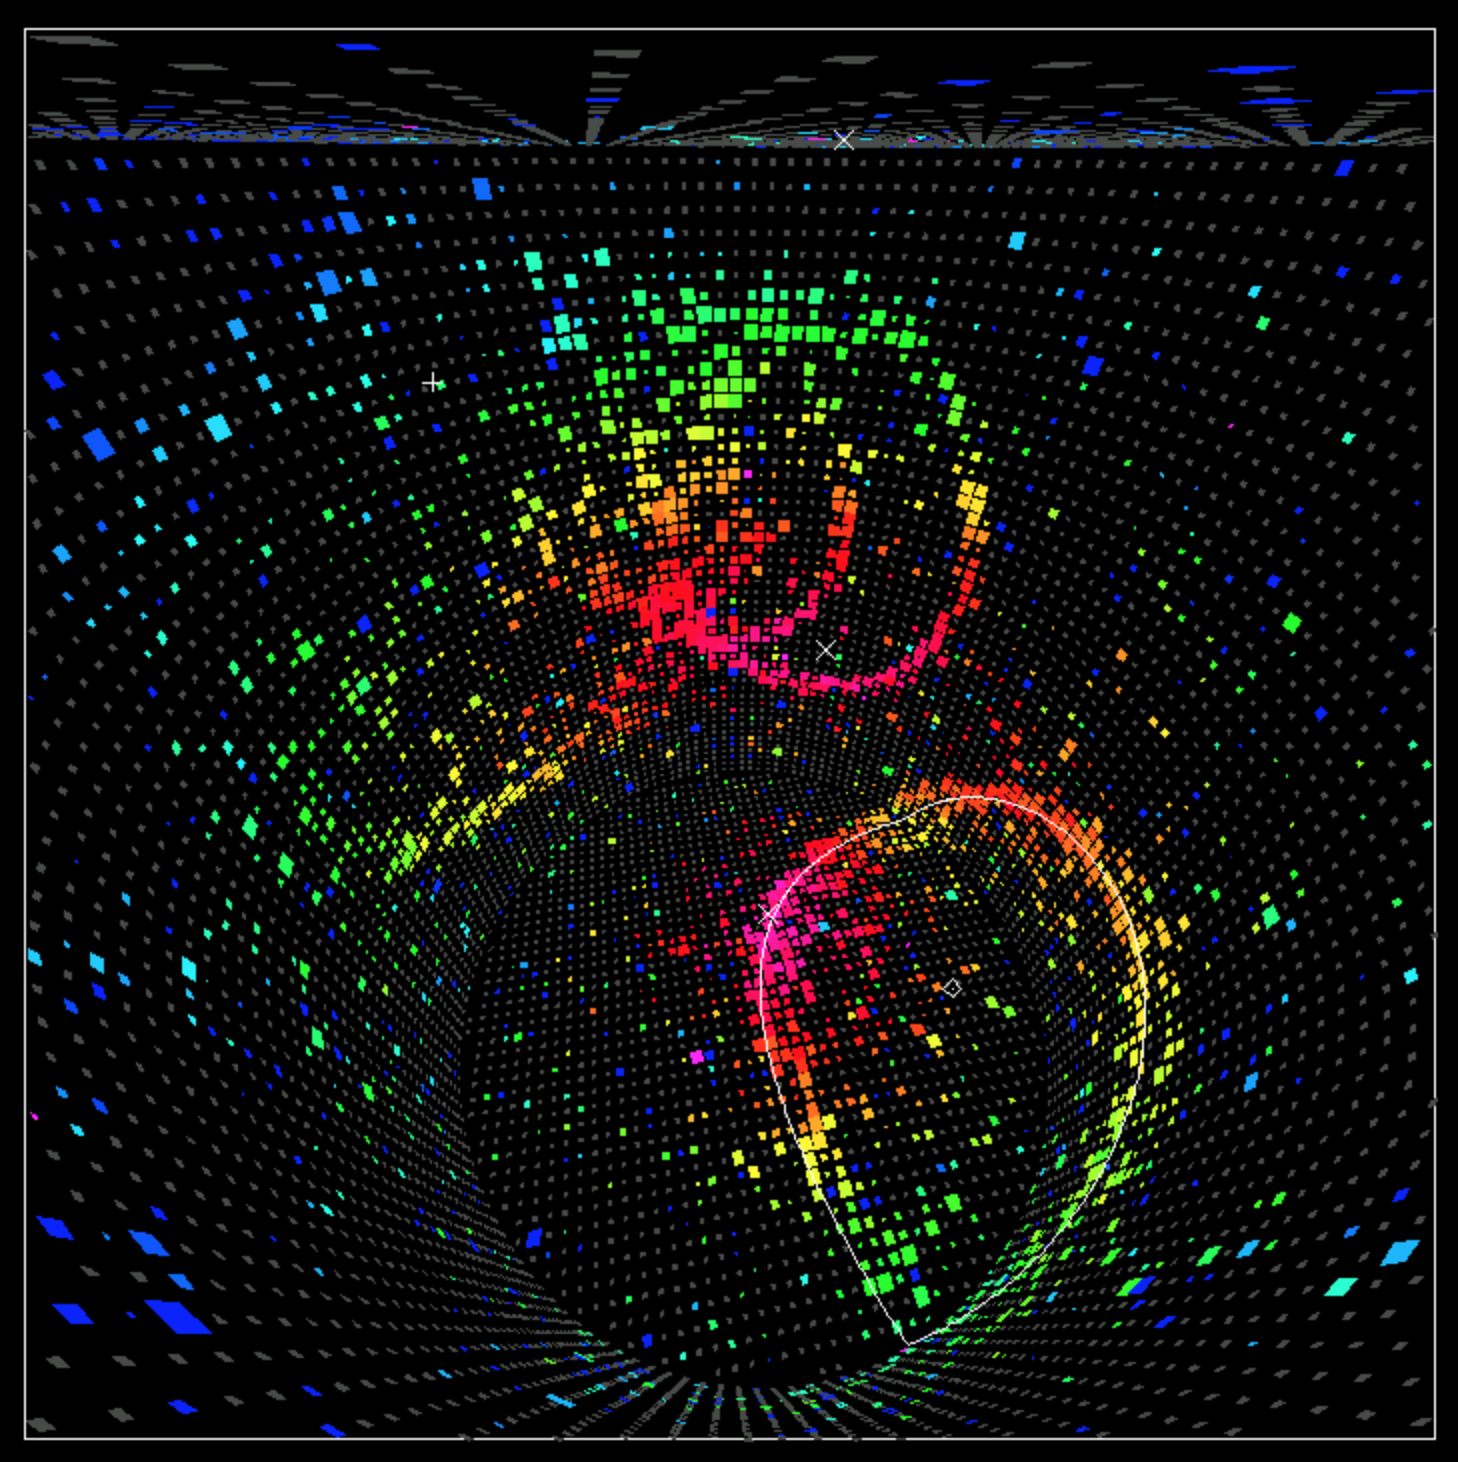
\includegraphics[width=5cm]{rings.png}
\caption{Proton decay candidate from Super-K data, event was rejected by analysis cuts. One candidate electron ring and two candidate photon rings from a pi-0 decay are visible. Graphic taken from "Images of Super-Kamiokande events from tscan", http://www.ps.uci.edu/~tomba/sk/tscan/pictures.html.}
\label{default}
\end{center}
\end{figure}

\subsection{$p \rightarrow K^{+}\bar{\nu}$}

SUSY GUT's add dimension 5 operators to the game, and predict a dominant proton decay mode of $p \rightarrow K^{+}\bar{\nu}$. In Super-K this signal is much more difficult to detect because the $K^{+}$ produced is under the cherenkov threshold of 749 MeV/c in water$^{[3]}$. As a result, the decay products of the kaon must be tagged instead. The exiting Kaon decays to a $\mu^{+}$ and neutrino 64 percent of the time, and a neutral and charged pion $\approx$ 36 percent of the time. There are 3 main methods to identify this proton decay channel.

\begin{enumerate}
\item If proton decay happens inside the oxygen nucleus, the remaining nucleus may be left in an excited state (this occurs roughly 65 percent of the time). This state then de-excites, emitting a prompt gamma ray with an average energy of 6 MeV. This method looks for the de-excitation gamma ray which precedes a single muon from the kaon decay. Figure 2 shows a simulated proton decay event in Super-K with a clearly visible muon ring, the prompt gamma ray can be seen in the PMT hit times in the lower right of the figure. 

\begin{figure}[htbp]
\begin{center}
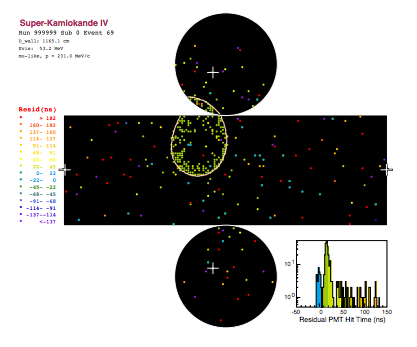
\includegraphics[width=7cm]{kaon_decay.png}
\caption{Simulated $p \rightarrow K^{+}\bar{\nu}$ in Super-K. Muon cherenkov ring visible, promp gamma ray hits are shown in cyan in the lower right. Graphic taken from [3].}
\label{default}
\end{center}
\end{figure}

\item Most $K^{+}$ stop in water, so a search for monoenergetic, 236 MeV/c $\mu^{+}$ from kaon decay would lead to an excess in the muon momentum distribution (Figure 3) from atmospheric neutrino backgrounds. 

\begin{figure}[htbp]
\begin{center}
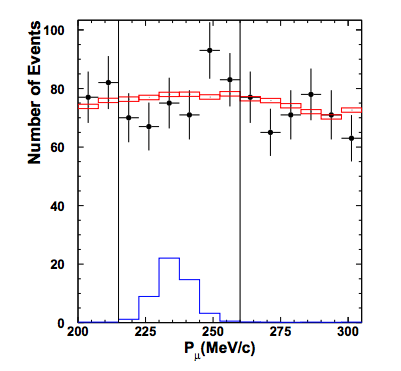
\includegraphics[width=9cm]{muon_momentum.png}
\caption{Muon momentum distribution from 260 kiloton years of exposure in Super-K. Black dots represent data, red boxes are the atmospheric neutrino monte-carlo, and blue is the proton decay monte-carlo. No excess is observed thus far. Graphic taken from [3].}
\label{default}
\end{center}
\end{figure}

\item Besides $K^{+} \rightarrow \mu^{+} \bar{\nu}$, the subdominant kaon decay mode is $K^{+} \rightarrow \pi^{+} + \pi^{0}$, where $\pi^{0}$ is produced with a momentum of 205 MeV/c. Reconstruction algorithms search for two cherenkov rings from the 2 $\pi^{0}$ photons, energy deposits in the backwards direction caused by the $\pi^{+}$ (the produced $\pi^{+}$ is only above cherenkov threshold by $\approx 50$ MeV/c), and a single Michel electron caused by the decay $\pi^{+} \rightarrow \mu^{+} \rightarrow e^{+}$ (schematic).
\end{enumerate}

Backgrounds for this proton decay channel come from atmospheric neutrino induced kaon production, charge current single $\pi^{0}$ production with a low momentum muon, and neutral current multi $\pi$ production. Background rates are predicted using the NEUT event generator. The dominant systematic uncertainties in the background come from the uncertainties in the neutrino flux and neutrino cross sections, which combined are on the order of 25-30 percent.

The signal efficiency and expected number of backgrounds for each of these 3 searches are: 7.9 percent and 0.39 events for prompt gamma detection, 33.7 percent and 579.4 events for muon momentum spectrum fit, and 8.2 percent and 0.56 events for the pion search. With over 300 kiloton years of exposure no significant excess is observed and a 90 percent C.L. lower lifetime limit of $\tau/B_{p\rightarrow K^{+}\bar{\nu}} > 6.6 \times 10^{33}$ years is placed on this channel$^{[3]}$. \newline



\section {DUNE}
The Deep Underground Neutrino Experiment, DUNE, is the next generation neutrino oscillation experiment to be built over the next 5-10 years. In addition to precisely measuring the mass hierarchy, the CP violating phase, $\delta$, and mixing angles, DUNE will be able to probe baryon number violating processes, the golden signal being proton decay. Unlike Super-K, DUNE is well suited for the proton decay mode $p \rightarrow K^{+}\bar{\nu}$, this is because of the LArTPC technology developed in preparation for the experiment$^{[4]}$.

\subsection{LAr Time Projection Chamber}
The DUNE far detector (FD) will be a 40 kiloton liquid argon detector 1450 meters underground at Sanford Underground Research Facility. In a Liquid Argon Time Projection Chamber (LArTPC), charged particles ionize Argon as they travel through the detector. Electronics are triggered to start recording by prompt scintillation light emitted by electron-ion recombinations and the decay of excimers (called S1 signal), and the electronic's clock starts. Liberated electrons are drifted to wire planes (anode) where their 2D location can be reconstructed. By examining the drift time, the 3rd dimension can also be reconstructed$^{[5]}$. This allows very precise reconstruction of charge particle tracks (Figure 4). 

\begin{figure}[htbp]
\begin{center}
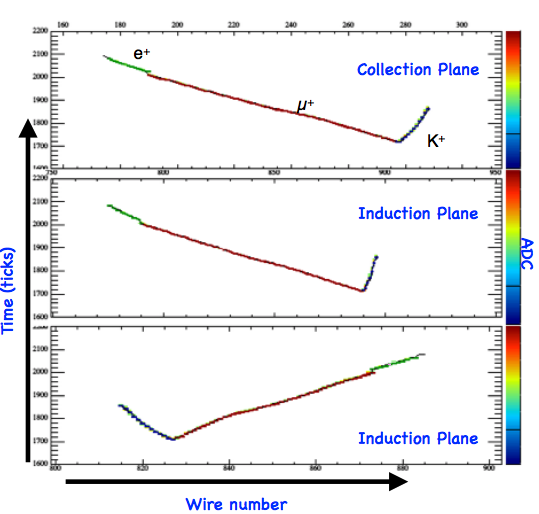
\includegraphics[width=7cm]{DUNE_kaon.png}
\caption{Simulated $p \rightarrow K^{+}\bar{\nu}$ in DUNE. Graphic taken from [5].}
\label{default}
\end{center}
\end{figure}
When a kaon is produced by proton decay, it emerges from the nucleus intact 97 percent of the time. The kaon emerging from this process is below cherenkov threshold in water, as discussed earlier, so only its decay products can be detected. In a LArTPC, the $K^{+}$ can be tracked, and identified via analysis of its energy loss profile and its kinetic energy measured by range. Additionally, all decay modes can be cleanly reconstructed. "With this level of detail, it is possible for a single event with an isolated kaon of the right momentum originating from a point within the fiducial volume, to provide overwhelming evidence for an observation of a proton decay."$^{[4]}$

The goal for DUNE is to fully reconstruct the kaon track and its decay products to unambiguously tag proton decay events. The key to this is kaon tracking efficiency, and particle identification. Default algorithms result in a 64 percent overall tracking efficiency for $K^{+}$, but this is highly momentum dependent (Figure 5). Kaon's are produced mono-energetically with momentum $\approx 339$ MeV/c, but interactions with the nucleus smear the final momentum. Different track reconstruction algorithms are being tested, and as of now, the efficiency is over 80 percent for kaons with momentum greater than 300 MeV/c.

\begin{figure}
\centering
\begin{minipage}{.5\textwidth}
  \centering
  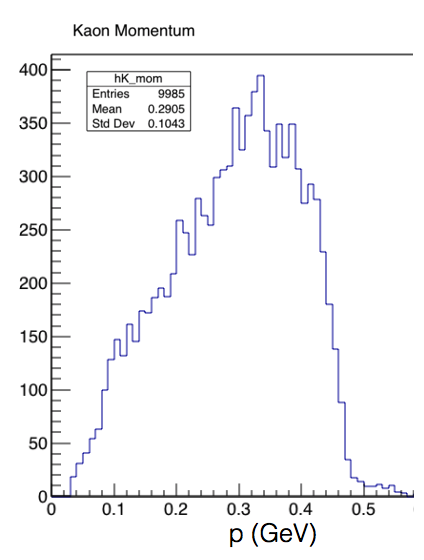
\includegraphics[width=.6\linewidth]{kaon_mom}
  \captionof{figure}{Kaon momentum distribution from 10,000 proton decays inside an Ar nucleus. Kaons are produced mono-energetically but their spectrum is smeared by interactions while exiting the nucleus. Graphic taken from [5]. }
  \label{fig:test1}
\end{minipage}%
\begin{minipage}{.5\textwidth}
  \centering
  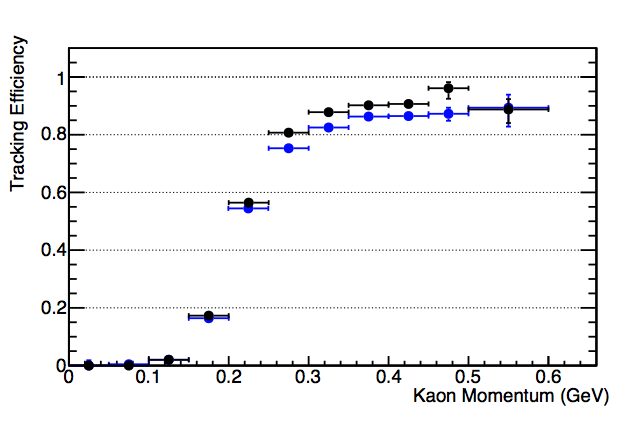
\includegraphics[width=1\linewidth]{kaon_tracking}
  \captionof{figure}{Kaon tracking efficiency as a function of kaon momentum. Blue is the default reconstruction algorithm, and black is an improved algorithm. Graphic taken from [4].}
  \label{fig:test2}
\end{minipage}
\end{figure}

Kaon identification is done with a combined analysis of timing, spatial reconstruction, decay products, and $\frac{dE}{dx}$ profile. Events selection for nucleon decay searches for 1) a tracked kaon 2) the muon from kaon decay 3) the Michel electron from muon decay. All daughter particles can be reconstructed and identified with high efficiency. For a more in depth look at analysis cuts and reconstruction efficiencies, see [4]. Even at this rudimentary level of kaon track reconstruction and particle identification, \textbf{efficiencies for low background reconstruction methods are an order of magnitude larger than in Super-K}.

Potential backgrounds for this channel in DUNE are atmospheric neutrino interactions, where a proton is misidentified as a kaon, kaons produced by muon interactions with rocks, and atmospheric neutrino kaon production. Proton/kaon discrimination is done by a combination of $\frac{dE}{dx}$, timing, and looking at decay products. Most kaons produced be cosmogenic muons are veto'd by looking for deposited energy near the edges of the detector. But, should a kaon enter the detector while an Argon nucleus undergoes beta decay, the light from the beta decay can "pull" the kaon track into the fiducial volume of the detector (Figure 7). About $10^3$ photo-electrons are expected on average for the initial scintillation signal for proton decay events, so monte-carlo studies are used to determine efficient cuts so as to remove events triggered by Ar beta decay$^{[4]}$$^{[5]}$. 

\begin{figure}[htbp]
\begin{center}
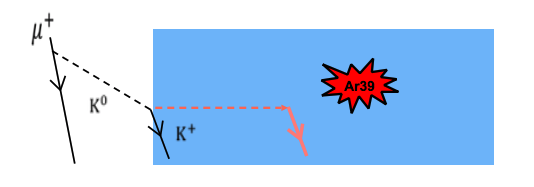
\includegraphics[width=9cm]{beta.png}
\caption{Cartoon of reconstructed kaon track being "pulled" into detector by Ar beta decay. Muon interacts with rock and produces neutral Kaon. Neutral Kaon undergoes charge exchange and produces charged kaon which enters the detector. Graphic taken from [5].}
\label{default}
\end{center}
\end{figure}

Kaon production by atmospheric neutrinos is a difficult background, as the rates are not well known. Luckily, MINERvA has only recently published the first high statistics neutrino induced charged kaon production analysis. This analysis was used to benchmark the current generation of neutrino interaction and final state interaction models. Results show consistent agreement with the GENIE neutrino cross section event generator$^{[6]}$, but this background needs to be studied more in the future.

Given the current state of reconstruction and analysis, DUNE has preliminarily evaluated its signal efficiency and background rates to calculate the partial lifetime sensitivity at 90 percent C.L for a 400 kiloton year exposure for this channel$^{[5]}$ (Figure 8).

\begin{figure}[htbp]
\begin{center}
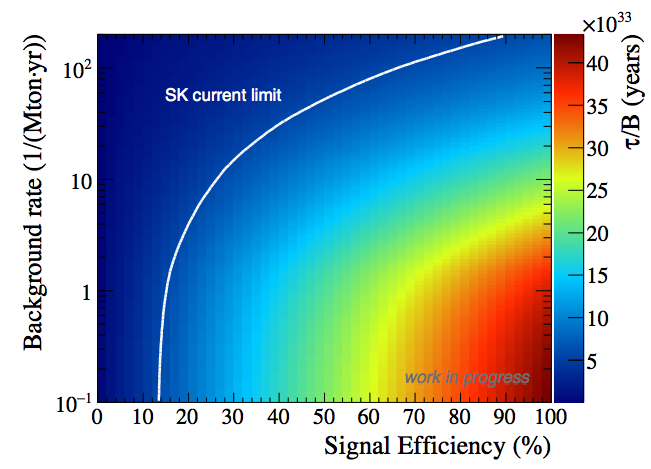
\includegraphics[width=9cm]{sensitivity.png}
\caption{Partial lifetime sensitivity vs Signal Efficiency (x axis) and Background rate (y axis). Graphic taken from [5].}
\label{default}
\end{center}
\end{figure}

Though there is much work to be done, DUNE seems poised to deliver an incredible measurement of the proton lifetime in this promising channel. 

\section{Bibliography}
\begin{enumerate}
\item Takhistov, V.,  "Review of Nucleon Decay Searches at Super-Kamiokande", arXiv:1605.03235v1 (2016)
\item Abe et al., "Search for proton decay via $p \rightarrow e^{+}\pi^{0}$ and $p \rightarrow \mu^{+}\pi^{0}$ in 0.31 megaton years exposure of the Super-Kamiokande water Cherenkov detector",  Physical Review D 95, 012004 (2017)
\item Abe et al., "Search for Proton Decay via $p \rightarrow K^{+}\nu$ using 260 kiloton year data of Super-Kamiokande",  arXiv:1408.1195v1 (2014)
\item DUNE Collab., "Far Detector Task Force Preliminary Report", Internal BNL report (2016)
\item Higuera, A., "DUNE Scientific Opportunities and Capabilities for Proton Decay Searches", Conference on Science at the Sanford Underground Research Facility (2017)
\item Marshall, C. "Measurement of neutral-current $K^{+}$ production by neutrinos using MINERvA",  arXiv:1611.02224v2 (2017)
\end{enumerate}



\end{document}